\chapter{数据库存储}

\begin{introduction}[期末考试提纲]
    \item RAID1、RAID5定义及其特性, 所适用的数据库应用场合
    \item 数据库的页结构和行结构
    \item LSM树、B+树
    \item 位图索引、按列存储
\end{introduction}

\section{存储介质}

\begin{figure}[H]
    \centering
    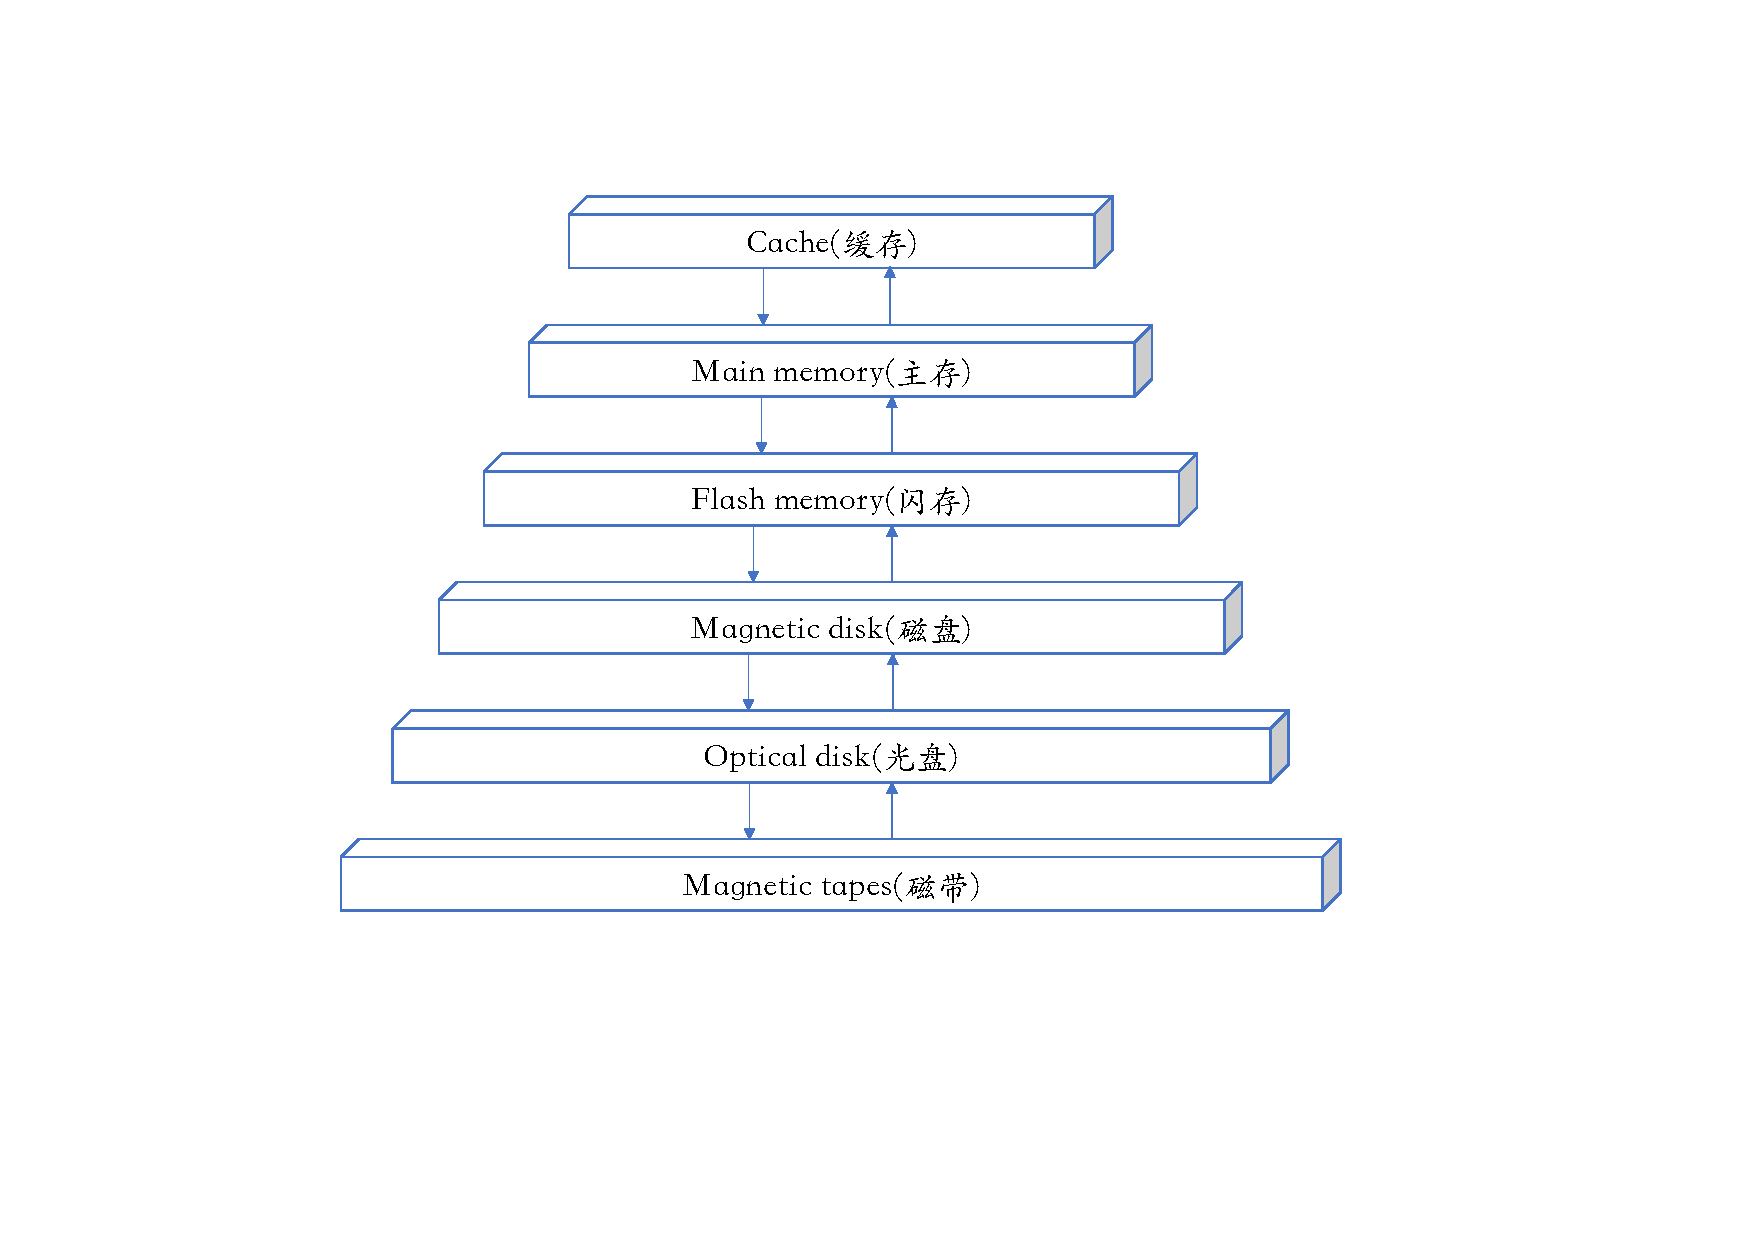
\includegraphics[width=.65\textwidth]{./figure/存储介质层次.pdf}
    \caption{物理存储介质的层次}
\end{figure}

局部性原理: CPU访问存储器时, 无论是存取指令还是存取数据, 所访问的存储单元都趋于聚集在一个较小的连续区域中.

\begin{itemize}
    \item 高速缓冲存储器(Cache): 最快最昂贵的存储介质; 很小, 由操作系统管理.
    \item 主存储器(main memory): 存放可被处理的数据的存储介质; 易失, 相对整个数据库太小.
    \item 快闪存储器(flash memory): 读性能类似主存, 写速度非常慢; 电子可擦除可编程只读存储器.
    \item 光学存储器(Optical storage): 只读(CD-ROM)、一次写多次读(WORM)、多次写(CD-RW).
    \item 磁带(tape): 顺序访问, 归档存储, 容量大, 价格便宜.
    \item 磁盘存储器(Magnetic-disk storage):
    \begin{itemize}
        \item 直接读取设备, 支持随机读取;
        \item 非易失联机数据存储设备;
        \item 访问数据时, 磁盘 $\to$ 内存;
        \item 修改后的数据, 内存 $\to$ 磁盘.
    \end{itemize}
\end{itemize}

